\documentclass{article}
\usepackage{graphicx}
\usepackage[utf8]{inputenc}
\usepackage[T1]{fontenc}
\usepackage[spanish]{babel}
\usepackage{amsmath}
\usepackage{listings}

\begin{document}

\title{Modelo de Ising en 2-D, usando CUDA}
\author{Jorge Fernandez-de-Cossio-Diaz}

\maketitle

\begin{abstract}
    Realizamos una simulación de Monte Carlo del modelo de Ising en 2 dimensiones usando CUDA.
    Comparamos la magnetización simulada con la solución analítica encontrada por Onsager en el límite termodinámico.
\end{abstract}

\section*{Introducción}

Este proyecto de CUDA implementa el algoritmo de Metrópolis para el modelo de Ising en 2-dimensiones.

Este modelo consiste de $N=L^2$ espines que toman valores $s_i=\pm 1$, colocados en una red cuadrada de dimensiones $L\times L$.
La energía de una configuración de este sistema es:
\begin{equation}
    E = -\sum_{(ij)} s_i s_j
\end{equation}
donde $(ij)$ recorre los pares de espines vecinos en la red.

En una simulación de Metrópolis de la dinámica de este sistema, un espín $i$ cambia de signo con una probabilidad
\begin{equation}
    \min\{1, \exp(-\beta\Delta E)\}
\end{equation}
donde $\Delta E$ es el costo energético del cambio de signo del espín $i$:
\begin{equation}
    \Delta E = 2\sum_{j\in\mathcal N(i)} s_i s_j
\end{equation}
$\beta=1/T$ es el inverso del a temperatura (en nuestras unidades la constante de Boltzmann es 1) y $\mathcal N(i)$ es el conjunto de espines vecinos a $i$ en la red cuadrada.

Se define la magnetización de una configuración de espines como:
\begin{equation}
    m=\frac{1}{N}\sum_i s_i
\end{equation}

Este sistema fue resuelto analícamente por Lars Onsager, en el límite termodinámico $N\rightarrow\infty$.
Onsager demostró la existencia de una transición de fase a la temperatura crítica:
\begin{equation}
    T_c = \frac{2}{\log(1 + \sqrt 2)} \approx 2.269185
\end{equation}
o $\beta_c=1/T_c\approx0.440687$.
Para $\beta\le\beta_c$, la magnetización es cero.
Para $\beta>\beta_c$, la magnetización es distinta de cero, y tiende a 1 a medida que $\beta$ crece.
Onsager encontró la siguiente expresión analítica para la magnetización, cuando $\beta\ge\beta_c$:
\begin{equation}
    m = [1-\sinh^{-4}(2\beta)]^{1/8}
    \label{eq:onsager}
\end{equation}

Programamos una simulación de Monte Carlo de este sistema en CUDA (fichero \texttt{cuda.cu}), con $N=1024$ espines ($L=32$).
El comportamiento se grafica en la figura \ref{fig:ising}, que muestra la solución analítica y la magnetización encontrada en las simulaciones.

\begin{figure}
    \centering
    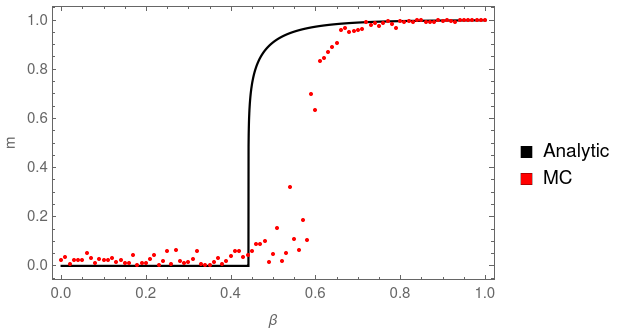
\includegraphics[width=0.9\textwidth]{Ising.png}
    \caption{\label{fig:ising} Magnetización del sistema a diferentes temperaturas obtenida por simulaciones de Monte Carlo, comparada con la magnetización analítica \eqref{eq:onsager}.}
\end{figure}

La discrepancia entre la solución analítica y las simulaciones se debe a que la solución de Onsager asume que el sistema es infinito ($N\rightarrow\infty$) mientras que las simulaciones son necesariamente en un sistema finito ($N=1024$).

Para reproducir estos resultados, compilamos \verb|ising.cu| y lo ejecutamos con los siguientes comandos:

\begin{verbatim}
    nvcc ising.cu -o ising --library=curand
    ./ising > ising.txt    
\end{verbatim}

A partir de estos datos (\verb|ising.txt|), la figura \ref{fig:ising} (\verb|Ising.png|) fue obtenida con el Notebook de Mathematica \verb|plot.nb|.

\end{document}